\section{Thermal shield vibrations}\label{sec:5:thermal-vibrations}

A spherical plate of radius $r_s$ clamped at its edge, can vibrate in distinct modes characterized by indices $(k,l)$, where $k \in [1,\infty)$ and $l \in [0, \infty)$.
The exact vibrational frequencies $\omega_{kl}$ and mode shapes $u_{kl}$ are described by Bessel functions.
In fact, one of the first occurrences of these functions is linked to Euler's study of vibrating perfectly flexible and infinitely thin membranes \cite{Dutka_1995}.
For a plate of a real material with density $\rho$ and thickness $d$, vibrations are described the differential equation \cite[p. 490]{Rao_2019}
\begin{equation}
  D \nabla^2\nabla^2 u = -\rho d \ddot{u}
\end{equation} 
where $D$, a flexural rigidity constant, is dependent on material properties of the plate like Youngs module $E$ and the Poisson ratio $\nu$ as
\begin{equation}
  D = \frac{d^3 E}{12(1-\nu^2)} .
\end{equation}
The general solution of this differential equation is expressed terms of Bessel functions as (derived in Ref. \cite[p. 490-495]{Rao_2019}) 
\begin{equation}
  u_{kl}(r, \theta, t) = \left[J_l(\beta_k r) - \frac{J_l(\beta_k r_s)}{I_l(\beta_k r_s)}I_l(\beta_k r)\right]\cos(l\theta+\phi_1)\sin(\omega_{kl}t+\phi_2)
\end{equation}
with
\begin{equation} \label{eq:5:vibration-frequency}
  \beta_k = \frac{\tilde{r}_k}{r_s} \quad \text{and} \quad \omega_{kl} = \frac{\tilde{r}_k^2}{r_s^2}\sqrt{\frac{D}{\rho d}} = \tilde{r}_k^2\frac{d}{r_s^2}\sqrt{\frac{E}{12\rho(1-\nu^2)}} .
\end{equation}
Here, $\tilde{r}_k$ is the $k$-th root of the equation
\begin{equation}\label{eq:5:bessel-zeros}
  J_l(\tilde{r}_k)I_{l+1}(\tilde{r}_k)+I_l(\tilde{r}_k)J_{l+1}(\tilde{r}_k) = 0 .
\end{equation}
The phases $\phi_1$ and $\phi_2$ 
are determined by initial conditions and represent rotational and temporal offsets.
The shape of the first 12 modes $(k,l)$ are shown in \cref{fig:5:vibrational-modes}.
\begin{figure}[!htbp]
  \centering
  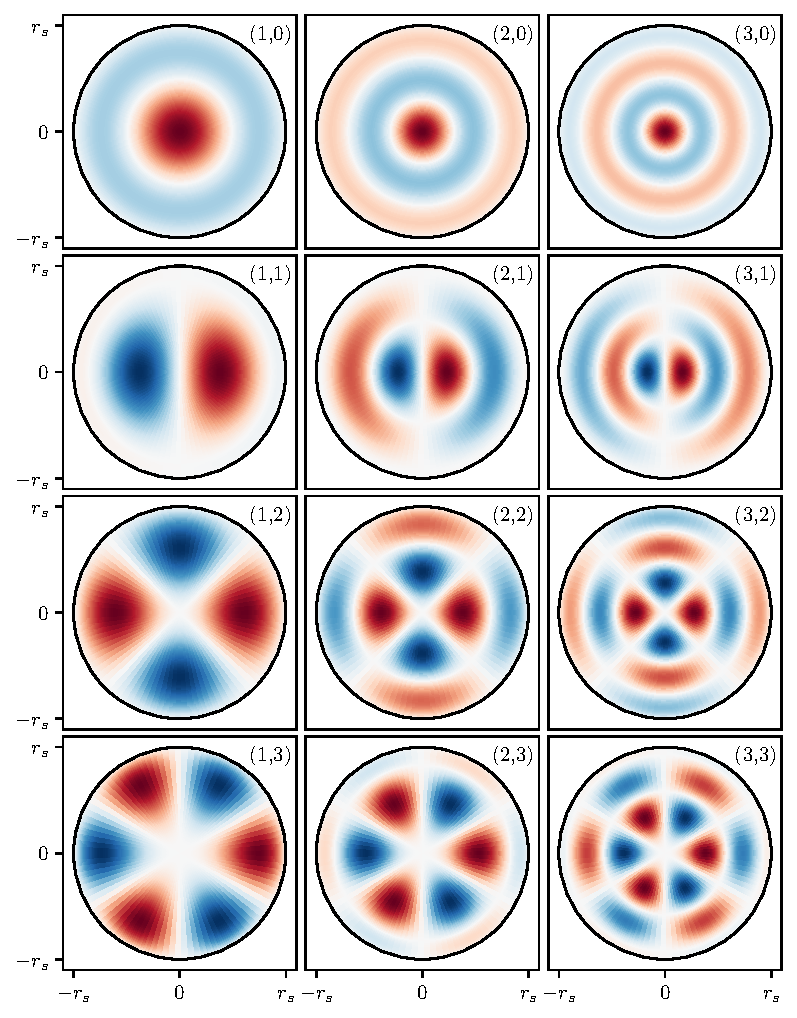
\includegraphics[width=\textwidth]{./../figures/vibrations/vibrational-modes-rd_bu.pdf}
  \caption{Shape of the first 12 modes $(k,l)$ ($k \geq 1$ and $l \geq 0$) of a vibrating spherical plate fixed at the edge with $r_s/d = 1000$.}
  \label{fig:5:vibrational-modes}
\end{figure}
In general, any possible vibration of the plates can be decomposed into a sum of these modes $u_{kl}$.
The amplitude $\op{z}$ depends on temperature $T$ and is treated as a quantum harmonic oscillator with frequency $\omega_{kl}$.
The expectation value of the amplitude $\avg{z\op{z}}$ is obviously zero and the variance $(\Delta \op{z})^2 = \avg{\op{z}^2} - \avg{\op{z}}^2$ at temperature $T$ is given by (derivation in \cref{apx:thermal-harmonic-oscillator})
\begin{equation}\label{eq:5:amplitude-variance}
  (\Delta \op{z}_{kl})^2_T = \frac{\hbar}{2\tilde{m}\omega_{kl}}\coth(\frac{\hbar \omega_{kl}}{2k_BT}) \approx \frac{k_B T}{\tilde{m}\omega_{kl}^2}
\end{equation}
where $\hbar\omega \ll k_B T$ was used in the last step and $k_B = 1.3806\times 10^{-23} \si{J/K}$ is the Boltzmann constant.
The \textit{effective mass} $\tilde{m}$ of the mode, considering the mode's shape, can intuitively be estimated by the average amplitude of the mode 
\begin{equation}\label{eq:5:effective-mass}
  \tilde{m} = m\frac{1}{\pi r_s^2}\int\limits_0^{r_s} \dd r \int\limits_0^{2\pi} r\dd\theta \, u_{kl}(r, \theta, t)
\end{equation}
with $m=\rho \pi r_s^2 d$ being the total mass of the plate.
The amplitude scales therefore as $\Delta z_{kl} \propto \omega^{-1}$ at high temperatures or for low frequencies.




\subsection*{The effect of infinite modes}
For a shield with radius $r_s = 1\si{cm} \gg R$ (referred to as the \q{large shield}) and thickness $d=100\si{nmm}$ made out of Copper with $E = 110\si{GPa}$ and $\nu = 1/3$, the vibrational frequencies for the first few modes are between $11.0\si{s^{-1}}$ for $(1,0)$ up to $1018\si{s^{-1}}$ for $(7,6)$.
These low frequencies result in vibrational energies $\hbar \omega$ that are much smaller than the thermal energy $k_B T$ at any reasonable temperature.
Consequently many vibrational modes are highly populated and even for temperatures of $10^{-6}\si{K}$, the first 600 modes are equally populated with probabilities close to $1/Z$, where $Z$ is the partition function
\begin{equation}
  Z = \sum_{m\in\{(k,l)\}} e^{-\beta \hbar \omega_m} .
\end{equation}

It is possible to determine the asymptotic increase of frequencies $\omega_{kl}$ for high modes $k,l \rightarrow \infty$.
Using the expansion of the Bessel functions for large arguments \cite[eq. 10.17.3]{DLMF}
\begin{equation}
  J_l(x) \sim \cos(x - \frac{l \pi}{2} - \frac{\pi}{4}) \quad \text{for} \ x \rightarrow \infty
\end{equation}
and of the modified Bessel functions for $x\rightarrow\infty$ \cite[eq. 10.40.1]{DLMF}
\begin{equation}
  I_l(x) \sim \frac{e^x}{\sqrt{2\pi x}} \quad \text{for} \ x \rightarrow \infty
\end{equation}
the asymptotic expansion of eq. \eqref{eq:5:bessel-zeros} can be expressed as
\begin{equation}
  \sim \frac{e^x}{\sqrt{2\pi x}} \left[\cos(x - \frac{l \pi}{2} - \frac{\pi}{4}) + \cos(x - \frac{l \pi}{2} - \frac{3 \pi}{4})\right] = 0 .
\end{equation}
For large $k\rightarrow\infty$, the zeros $\tilde{r}_k$ occur periodically.
For large orders $l\rightarrow \infty$, the Bessel functions $J_l$ scale like \cite[eq. 10.19.1]{DLMF}
\begin{equation}
  J_l(x) \sim \frac{1}{\sqrt{l}} \left(\frac{ex}{2l}\right)^l \quad \text{for} \ l \rightarrow \infty
\end{equation}
implying that the first zero shift outwards with $\tilde{r}_1 \gtrsim 2l/e$.
For high modes $k$ and $l$ this results in an linear asymptotic distribution of zeros and thus, the frequencies $\omega_{kl}$ scale in the order of $\mathcal{O}((k + l)^2)$.

Since the amplitude scales inversely with frequency $\Delta z_{kl} \propto 1/\omega_{kl}$, higher modes exhibit a quadratic decrease in amplitude.
Additionally, the shape function $u_{kl}$ of higher modes has more bulges, limiting the amplitude further as the available shield-material is distributed over smaller segments of the plate.
These effects combine to ensure that higher-order modes have minimal contributions, allowing numerical calculations to focus on the first few modes.
Nevertheless, the influence of infinitely many modes can still be approximated asymptotically using the scaling behavior of $\omega_{kl}$.

It is also interesting to consider the scaling of the amplitudes $\Delta z$ for shields with varying sizes $r_s$.
According to eq. \eqref{eq:5:vibration-frequency}, the frequency $\omega$ increases quadratically as the shield radius $r_s$ decreases.
Simultaneously, the effective mass $\tilde{m}$ in eq. \eqref{eq:5:effective-mass} scales also quadratically with the shield's size, consequently resulting in linear dependence of $\Delta z \sim r_s$ for large temperatures and/or low modes.